\documentclass[titlepage,10pt,letter]{report}
\usepackage[toc,page]{appendix}
\usepackage{pdflscape}
\usepackage{extsizes}			\usepackage{bm}
\usepackage[english]{babel}		\usepackage{amsmath}
\usepackage{amsfonts}			\usepackage{amssymb}
\usepackage{graphicx}			\usepackage{epsfig}
\usepackage{sectsty}			\usepackage{booktabs}
\usepackage{floatrow}			\floatsetup[table]{capposition=top}	
\usepackage{siunitx}			\usepackage{caption}
\usepackage{subcaption}			\usepackage{listings}
\usepackage{authblk}			\usepackage{rotating}
\usepackage{multicol}			\usepackage{multirow}
\usepackage{mathrsfs}			\usepackage[useregional]{datetime2}
\PassOptionsToPackage{hyphens}{url}
\usepackage{hyperref}			\hypersetup{colorlinks = true, citecolor = OliveGreen}
\usepackage[dvipsnames]{xcolor}	\usepackage{pdfpages}
\usepackage{soul}				\usepackage{enumitem}	
\usepackage{indentfirst}		\usepackage{tcolorbox}
\usepackage{color, colortbl}
%\usepackage[numbered,framed]{mcode}

\def\thesection{\arabic{section}}	\def\theequation{\arabic{equation}}

\setlength{\textwidth}{6.5in}		\setlength{\textheight}{9.0in}
\setlength{\oddsidemargin}{0in}		\setlength{\topmargin}{-0.5in}
%% New Commands
\newcommand{\p}{\partial}
\newcommand{\e}[1]{\ensuremath{\times 10^{#1}}}
\newcommand{\abs}[1]{\left| #1 \right|}
\newcommand{\paren}[1]{\left( #1 \right)}
\newcommand{\bracket}[1]{\left[ #1 \right]}
\newcommand{\cbracket}[1]{\left{ #1 \right}}
\newcommand{\at}[2]{\left. #1 \right|_{#2}}
\newcommand{\highlightbox}[2]{\colorbox{#1}{$\displaystyle #2$}}
\newcommand{\hlcolor}[2]{\sethlcolor{#1}\hl{#2}}
\newcommand{\F}{^\circ F}
\newcommand{\C}{^\circ C}
\newcommand{\inch}{^{\prime \prime}}

%% equation, figure and tabel number with section number
\usepackage{chngcntr}
\counterwithin{figure}{chapter}
\counterwithin{table}{chapter}
\numberwithin{equation}{chapter}
%% These settings can be changed
\setlength{\parindent}{0.5in}
\setlength{\parskip}{0.5em}
\setcounter{section}{0}


\begin{document}
\begin{titlepage}
	\centering
	\vspace*{2.5in}
	{\huge\textbf{UCSD Design/Build/Fly\\Foamcutter Guide} \par}
	
	\vspace{2.5in}
	{\large Yuting Huang \\
		\href{mailto:ythuang96@gmail.com}{ythuang96@gmail.com}} \\
	\vspace{1.5in}
	{\large
		Updated: \\
		\today }
	\vspace{1in}
\end{titlepage}

\newpage
\tableofcontents
\newpage


\chapter{Preparations}
\section{Laptop Setup}

The foamcutter is controlled by a Raspberry Pi3. In order to communicate with the Pi, a Windows laptop has to install \textbf{PuTTY} (or similar) for secure shell (ssh) connection to the Pi, and \textbf{WinSCP} (or similar) for graphical file management. \textbf{This setup process is only required once per laptop.} A Linux laptop have ssh capability built in, therefore, no software required.

\subsection{PuTTY Setup}

\noindent Please follow the following steps for install and setup of PuTTY:

\begin{enumerate}[noitemsep,topsep=0pt]
	\item Download PuTTY at \href{https://www.putty.org/}{https://www.putty.org/} then install.
	\item Launch PuTTY and a window similar to fig~\ref{fig:putty1} below should show up:
	\begin{figure} [H]
		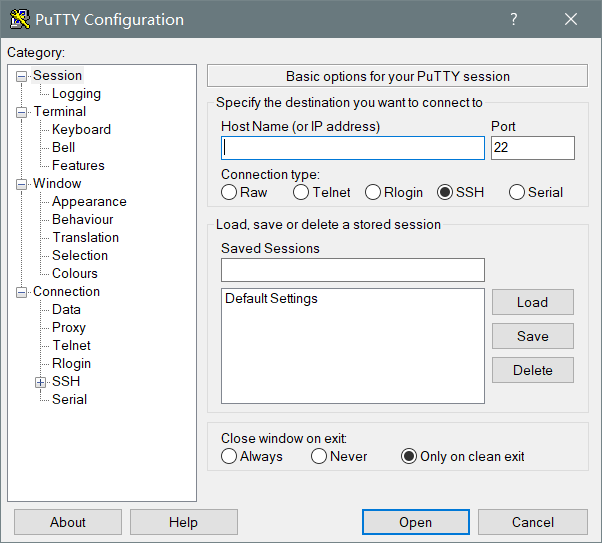
\includegraphics[width = 0.6\linewidth]{./Figures/Laptop_Setup/putty1.png}
		\caption{PuTTY Launch Window}
		\label{fig:putty1}
	\end{figure}
	\item As shown in fig~\ref{fig:putty2} below, in the HostName field, enter ``foamcutter.local", then make sure Connection type is SSH. Next, in Saved Session field, enter ``foamcutter", and lastly, click save.
	\begin{figure} [H]
		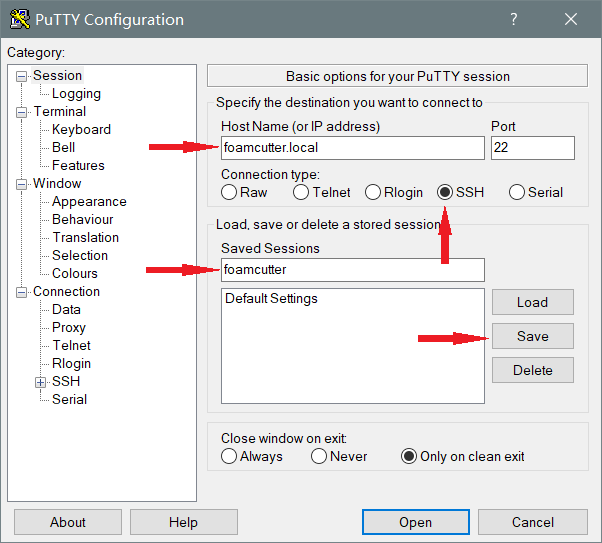
\includegraphics[width = 0.6\linewidth]{./Figures/Laptop_Setup/putty2.png}
		\caption{PuTTY Setup}
		\label{fig:putty2}
	\end{figure}
	\item The session with name ``foamcutter" should show up in Saved Session as shown in fig~\ref{fig:putty3} below, and the PuTTY setup is completed.
	\begin{figure} [H]
		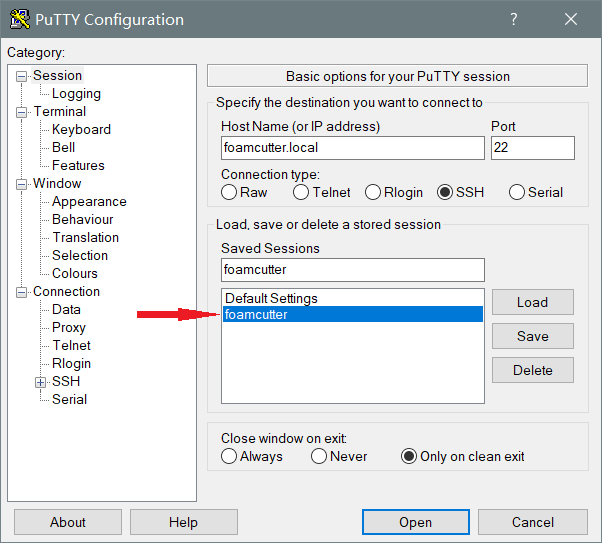
\includegraphics[width = 0.6\linewidth]{./Figures/Laptop_Setup/putty3.png}
		\caption{Saved PuTTY Session}
		\label{fig:putty3}
	\end{figure}
\end{enumerate}

\subsection{WinSCP Setup}

\noindent Please follow the following steps for install and setup of WinSCP:

\begin{enumerate}[noitemsep,topsep=0pt]
	\item Download WinSCP at \href{https://winscp.net/eng/download.php}{https://winscp.net/eng/download.php} then install.
	\item Launch WinSCP and a window similar to fig~\ref{fig:winscp1} below should show up:
	\begin{figure} [H]
		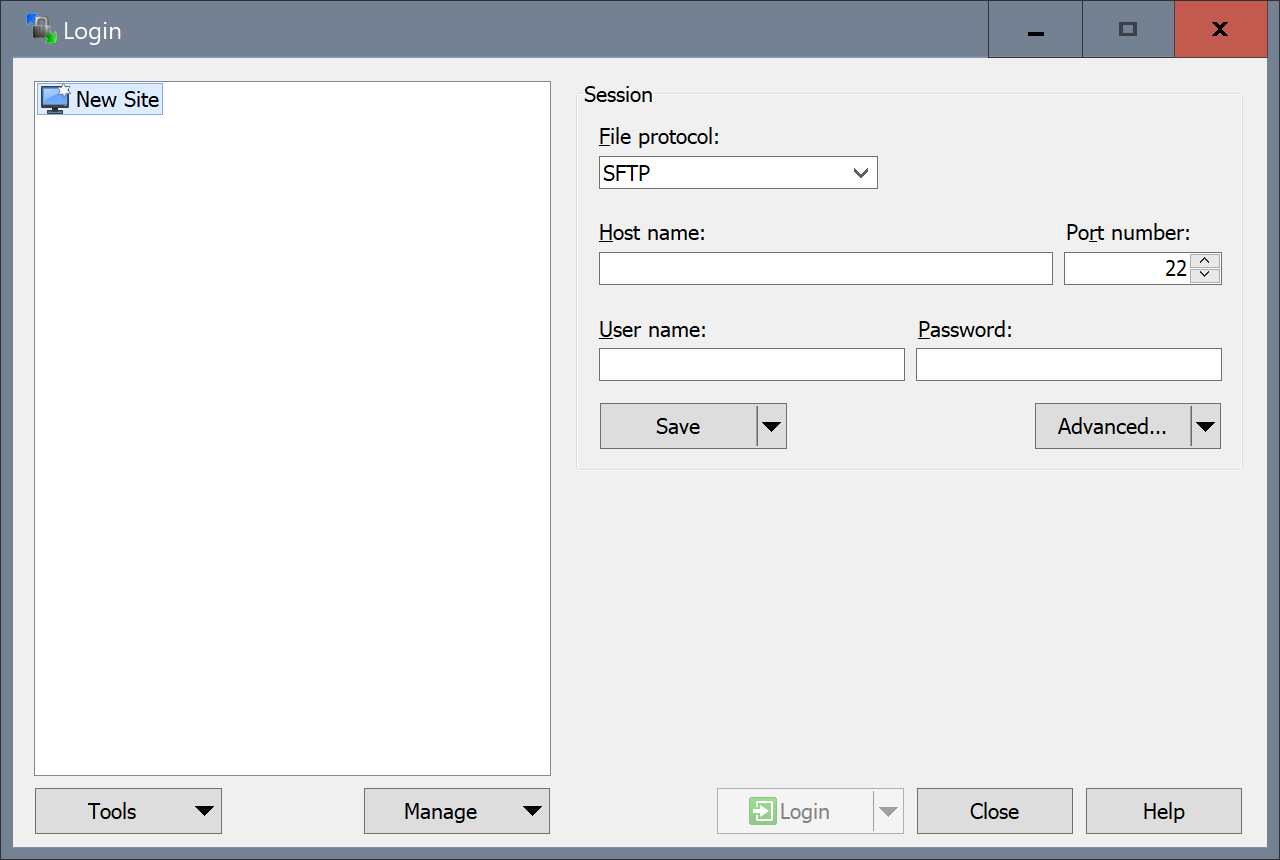
\includegraphics[width = 0.6\linewidth]{./Figures/Laptop_Setup/winscp1.png}
		\caption{WinSCP Launch Window}
		\label{fig:winscp1}
	\end{figure}
	\item As shown in fig~\ref{fig:winscp2} below, make sure the protocol is ``SFTP", then enter ``foamcutter.local" for the host name, ``pi" for the user name, and ``ucsdaiaadbf" for the password.
	\begin{figure} [H]
		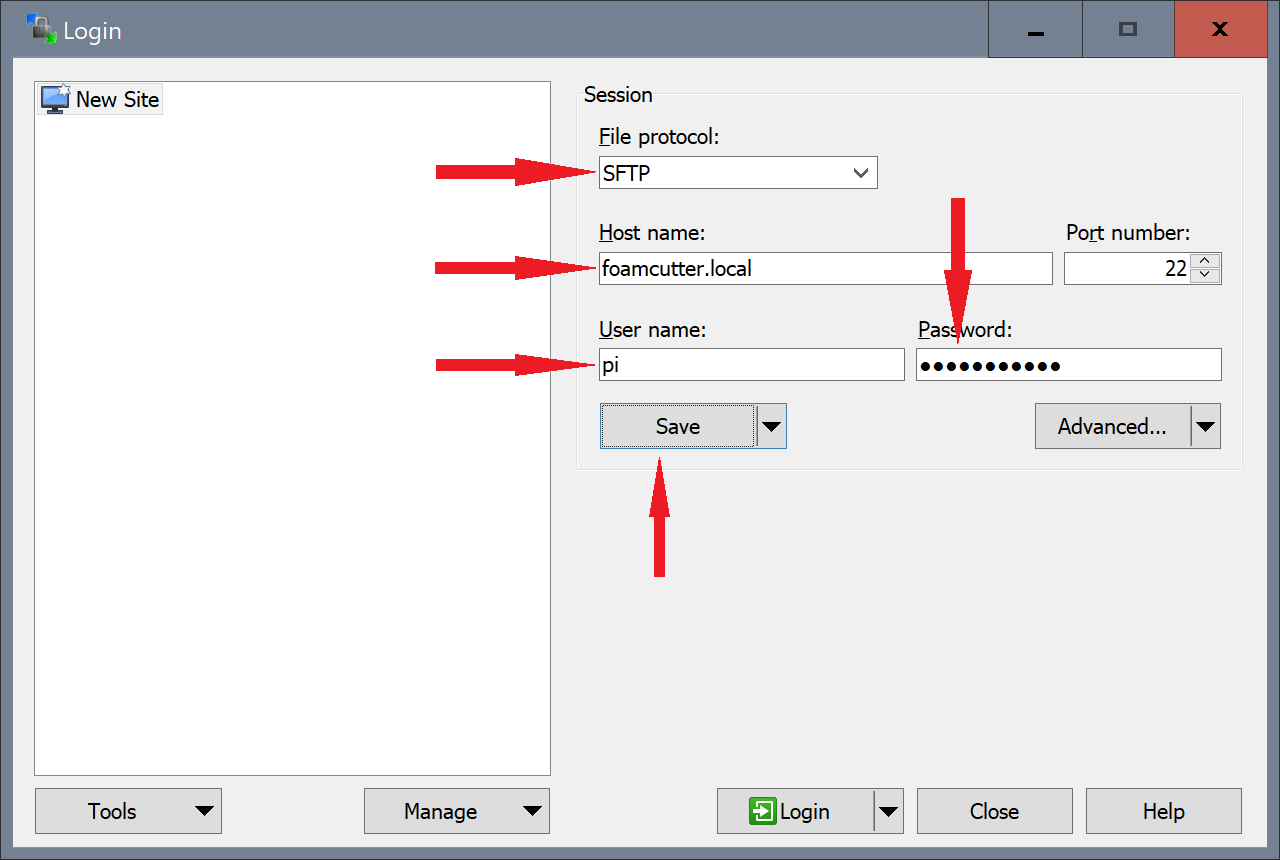
\includegraphics[width = 0.6\linewidth]{./Figures/Laptop_Setup/winscp2.png}
		\caption{WinSCP Setup}
		\label{fig:winscp2}
	\end{figure}
	\item Click save, and a window shown in fig~\ref{fig:winscp3} below should pop up. Both ``Save password" and ``Create desktop shortcut" are recommended. Click ``OK" and the setup for WinSCP is completed. 
	\begin{figure} [H]
		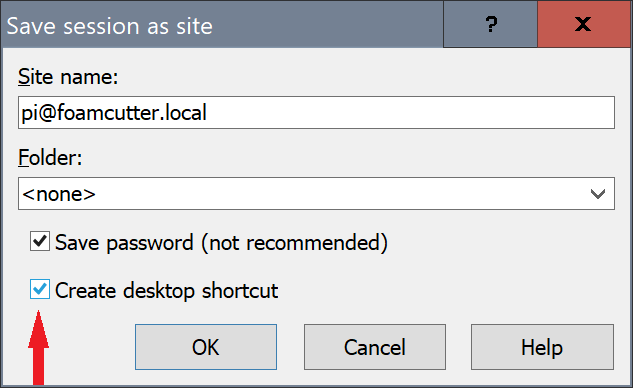
\includegraphics[width = 0.6\linewidth]{./Figures/Laptop_Setup/winscp3.png}
		\caption{WinSCP Setup continued}
		\label{fig:winscp3}
	\end{figure}
\end{enumerate}

\newpage

\section{G-Code Generation}
\subsection{G-Code for Wing}
\begin{itemize}[noitemsep,topsep=0pt] 
	\item Download the airfoil coordinates at \href{http://m-selig.ae.illinois.edu/ads/coord_database.html#S}{http://m-selig.ae.illinois.edu/ads/coord\_database.html\#S}
	
\end{itemize}

\subsection{G-Code for General Shapes}
\begin{tcolorbox}
	{\Large
		\noindent Key Points:
		\begin{itemize}[noitemsep,topsep=0pt]
			\item Make sure to increase AutoCAD precision;
			\item Make sure to scale the drawing by 25.4 in AutoCAD if the SolidWorks file is in inches;
			\item Make sure to run ``Explode'' command in AutoCAD;
			\item Make sure there are no overlapping lines;
			\item Make sure to convert spline to polyline in AutoCAD and explode again.
		\end{itemize}
	}
\end{tcolorbox}

\begin{enumerate}[noitemsep,topsep=0pt]
	\item Export the projection of the top or side (or both) profiles from SolidWorks into .dxf files, the steps are demonstrated with the payload bay shown in fig~\ref{fig:sw1} below.
	\begin{figure} [H]
		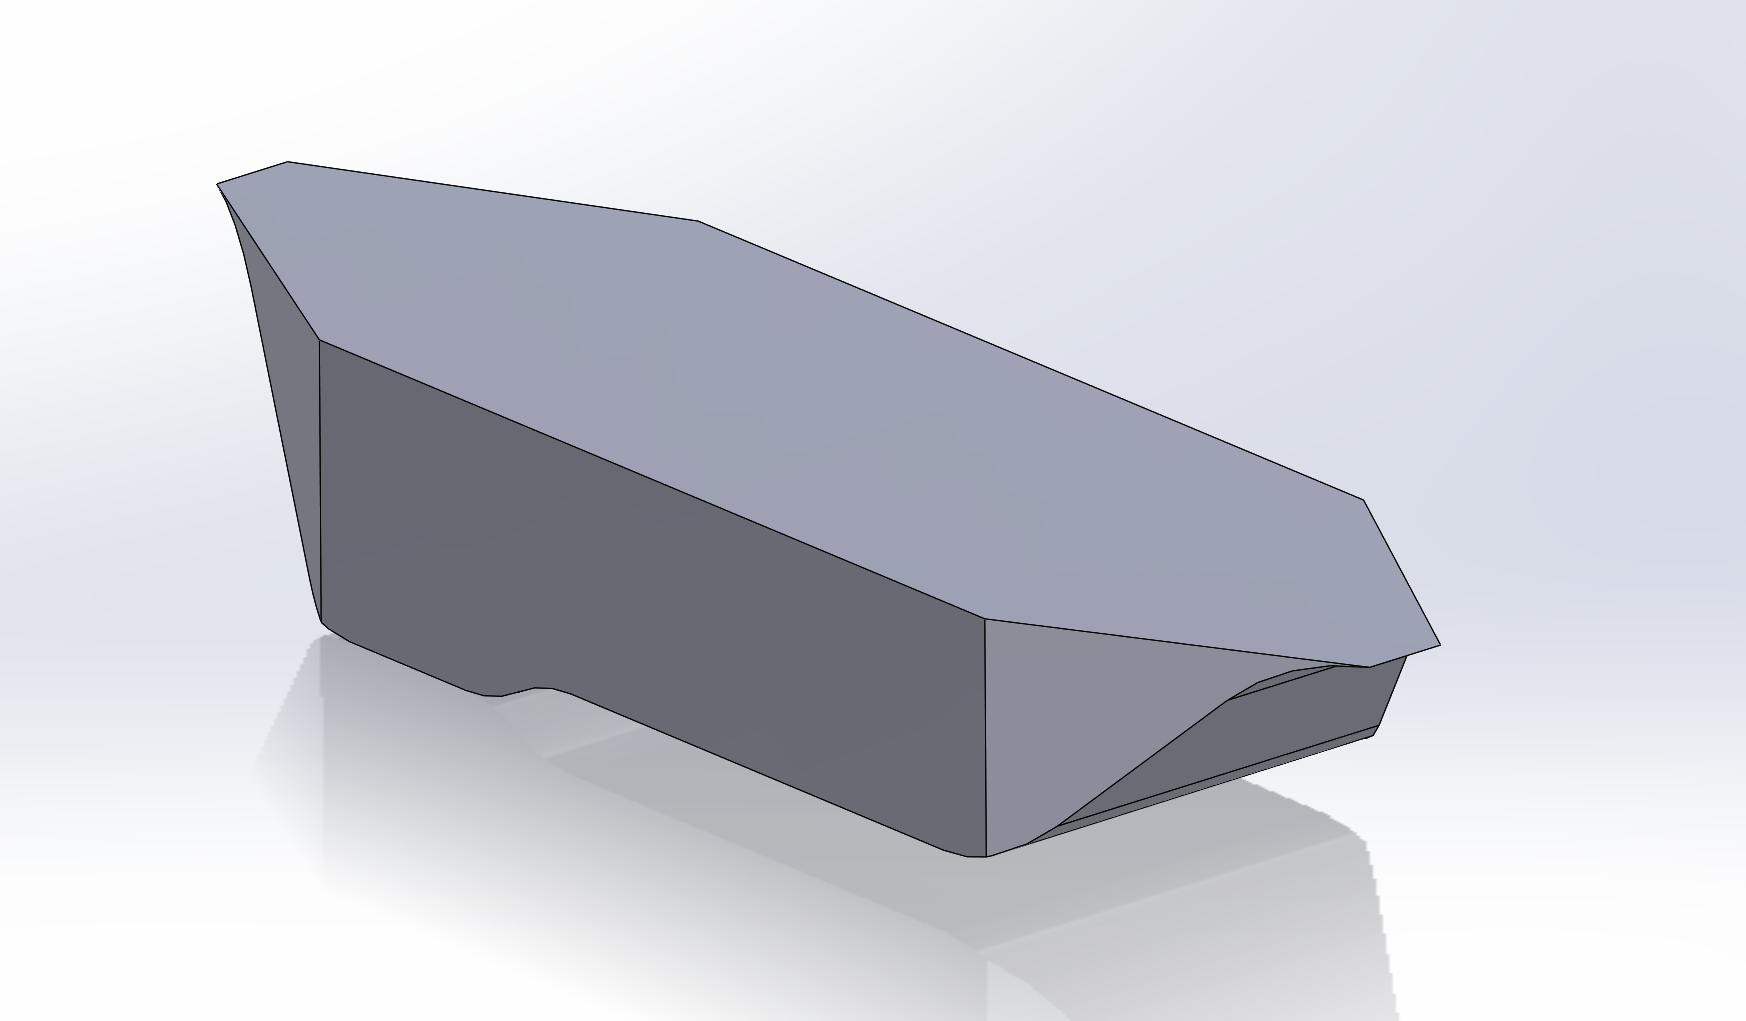
\includegraphics[width = 0.6\linewidth]{./Figures/general_shape/sw1.png}
		\caption{Sample Payload Bay}
		\label{fig:sw1}
	\end{figure}
	\begin{itemize}[noitemsep,topsep=0pt]
		\item The projection of the side profile can be obtained by slicing the part vertically in the center: go to ``Insert $\rightarrow$ Features $\rightarrow$ Split'' as shown in fig~\ref{fig:sw2} below:
		\begin{figure} [H]
			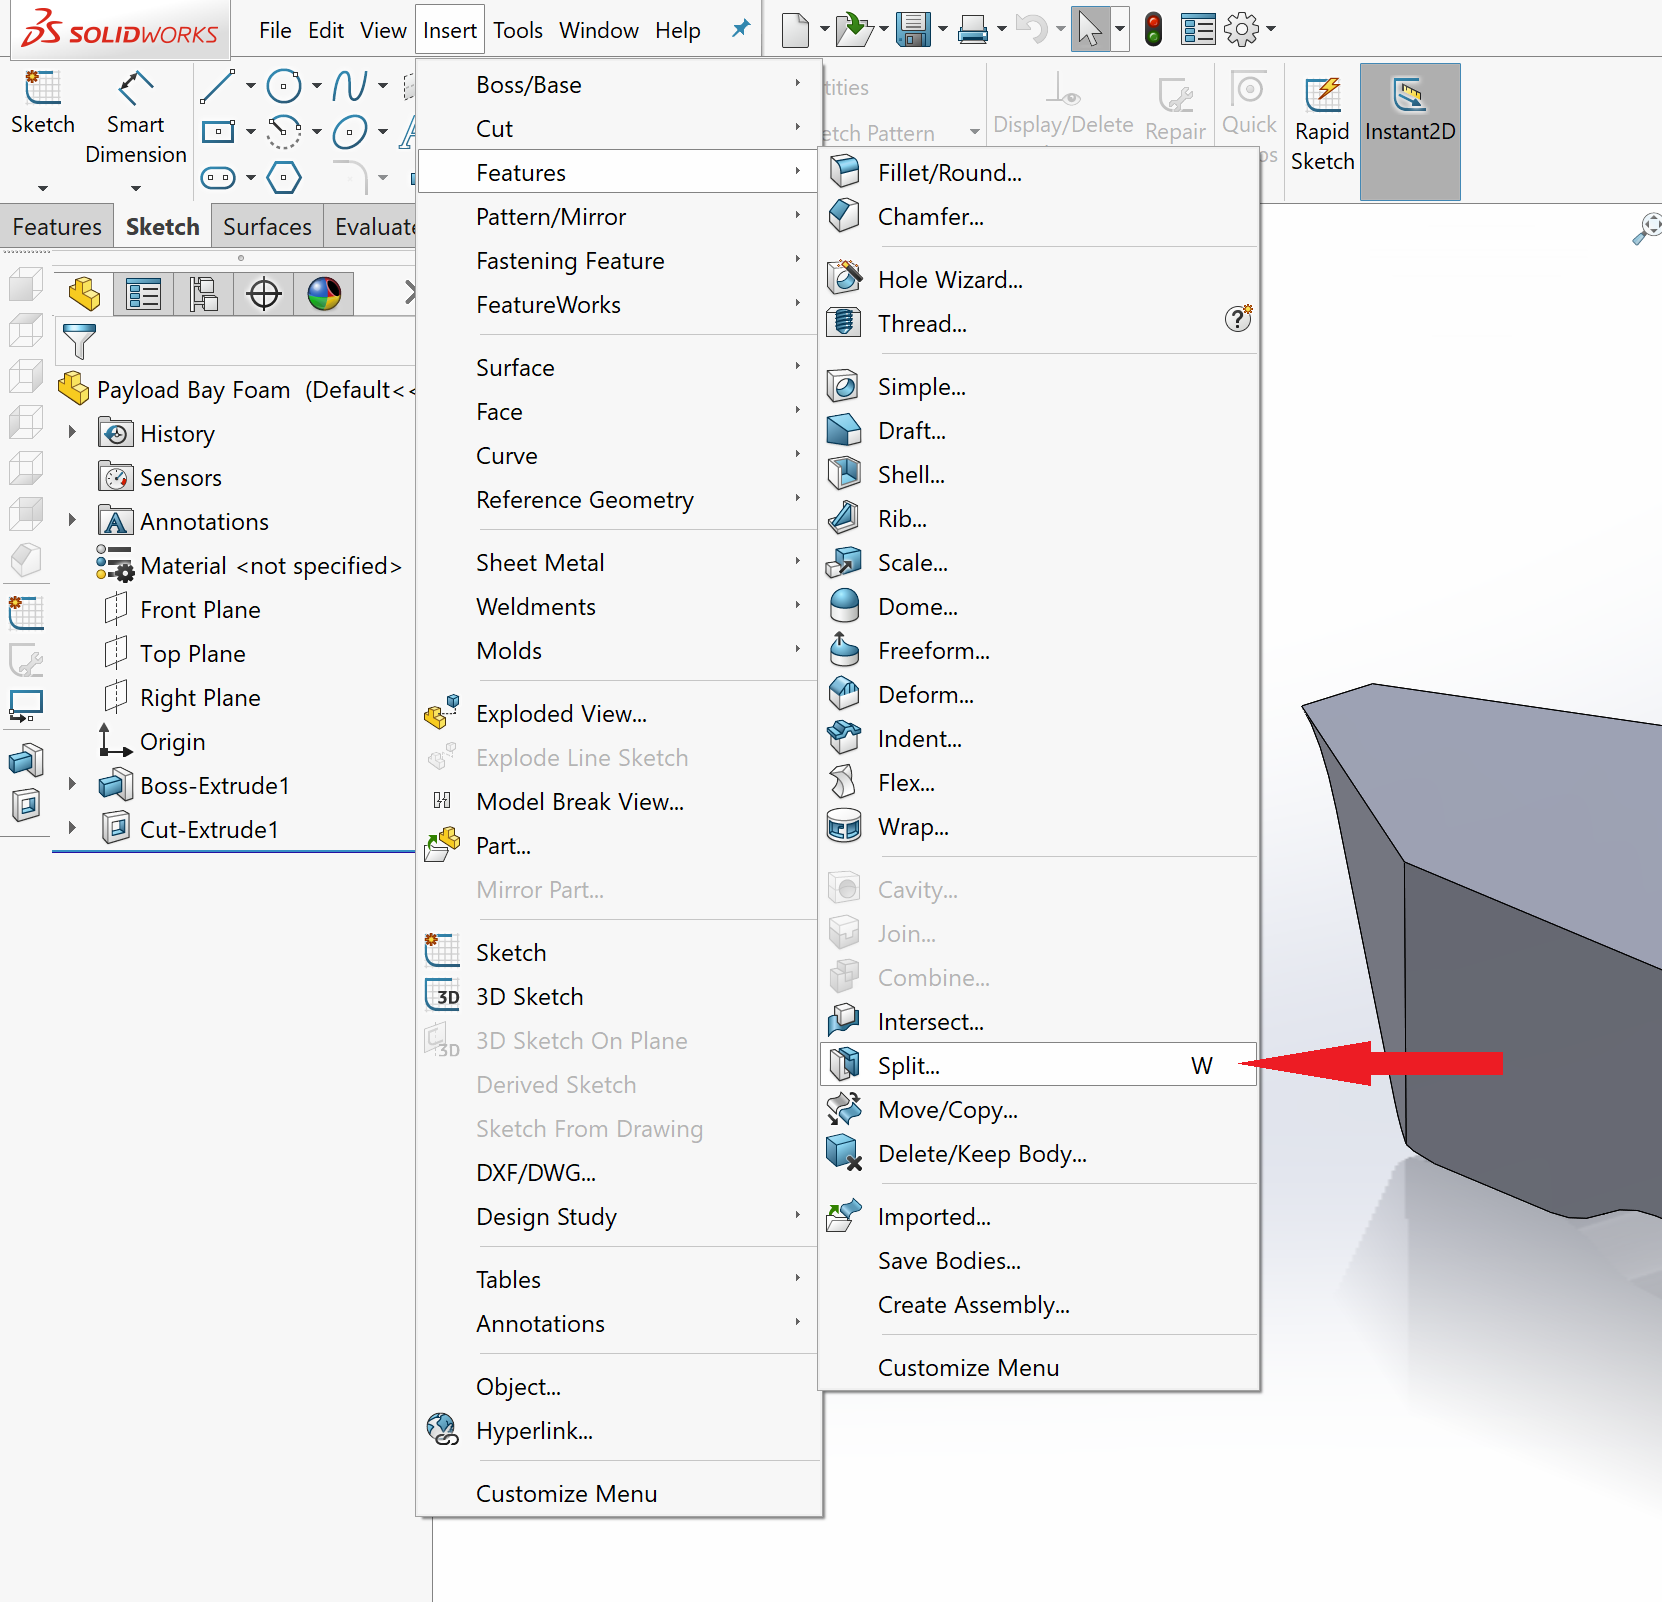
\includegraphics[width = 0.6\linewidth]{./Figures/general_shape/sw2.png}
			\caption{SolidWorks Split Command}
			\label{fig:sw2}
		\end{figure}
	
		\item In the pop up window, as shown in fig~\ref{fig:sw3} below, in ``Trim Tools'' selected the desired plane (the front plane in this case) then click ``Cut Body''. In the ``Resulting Bodies'' box, select one of the resulting bodies. Lastly, make sure the ``Consume cut bodies'' check box is selected, and click the top left green check mark. This will delete the selected half of the part (the brown half in fig~\ref{fig:sw3}).
		\begin{figure} [H]
			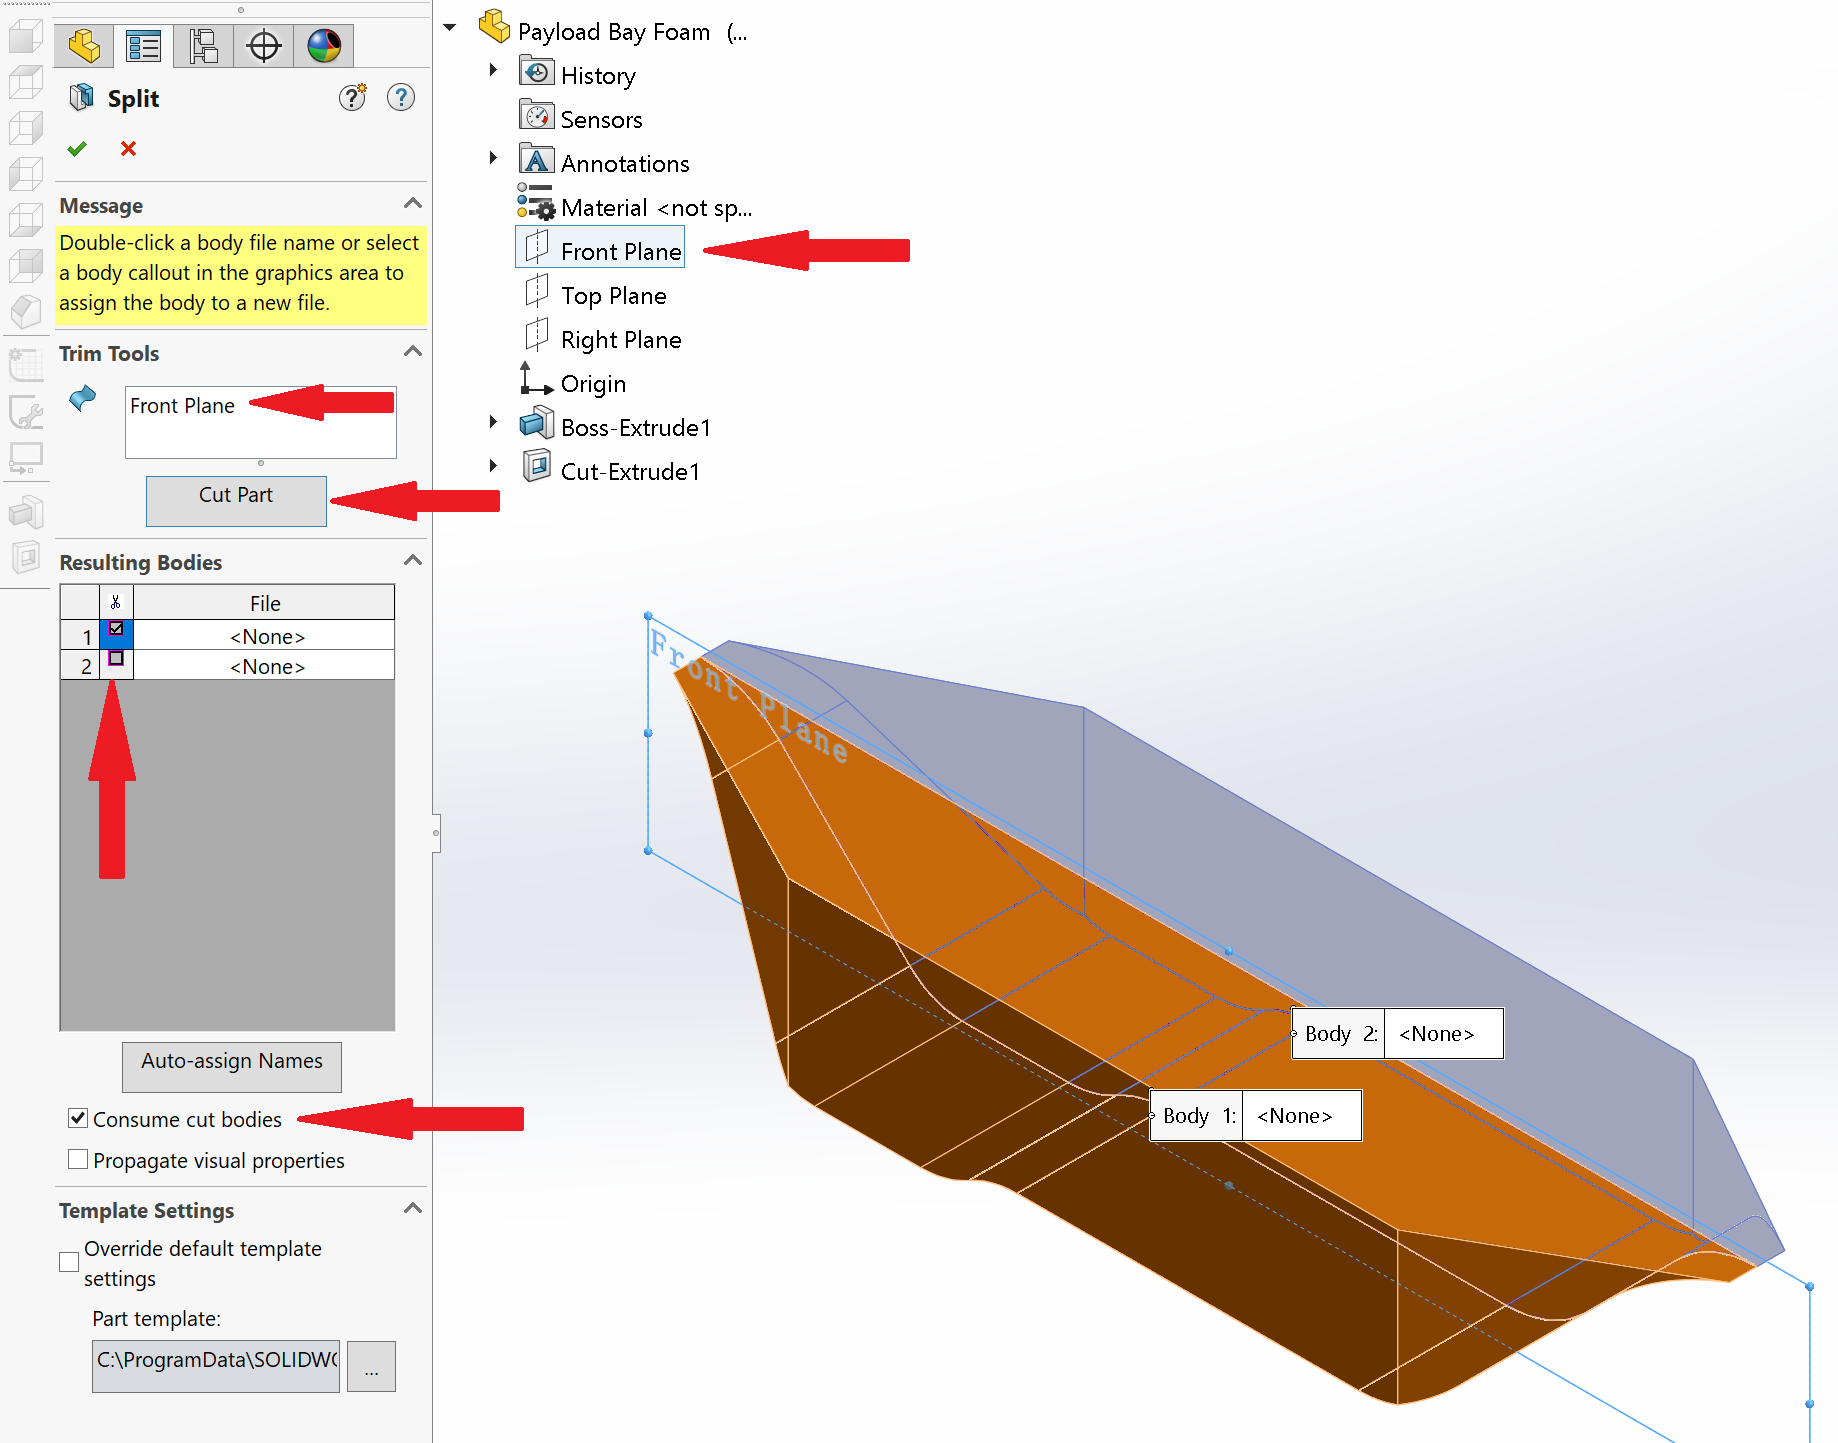
\includegraphics[width = 0.9 \linewidth]{./Figures/general_shape/sw3.png}
			\caption{SolidWorks Split Menu}
			\label{fig:sw3}
		\end{figure}
	
		\item Right click on the cut plane and select ``Export to DXF/DEG'' to export the projection of the side profile as shown in fig~\ref{fig:sw4} below:
		\begin{figure} [H]
			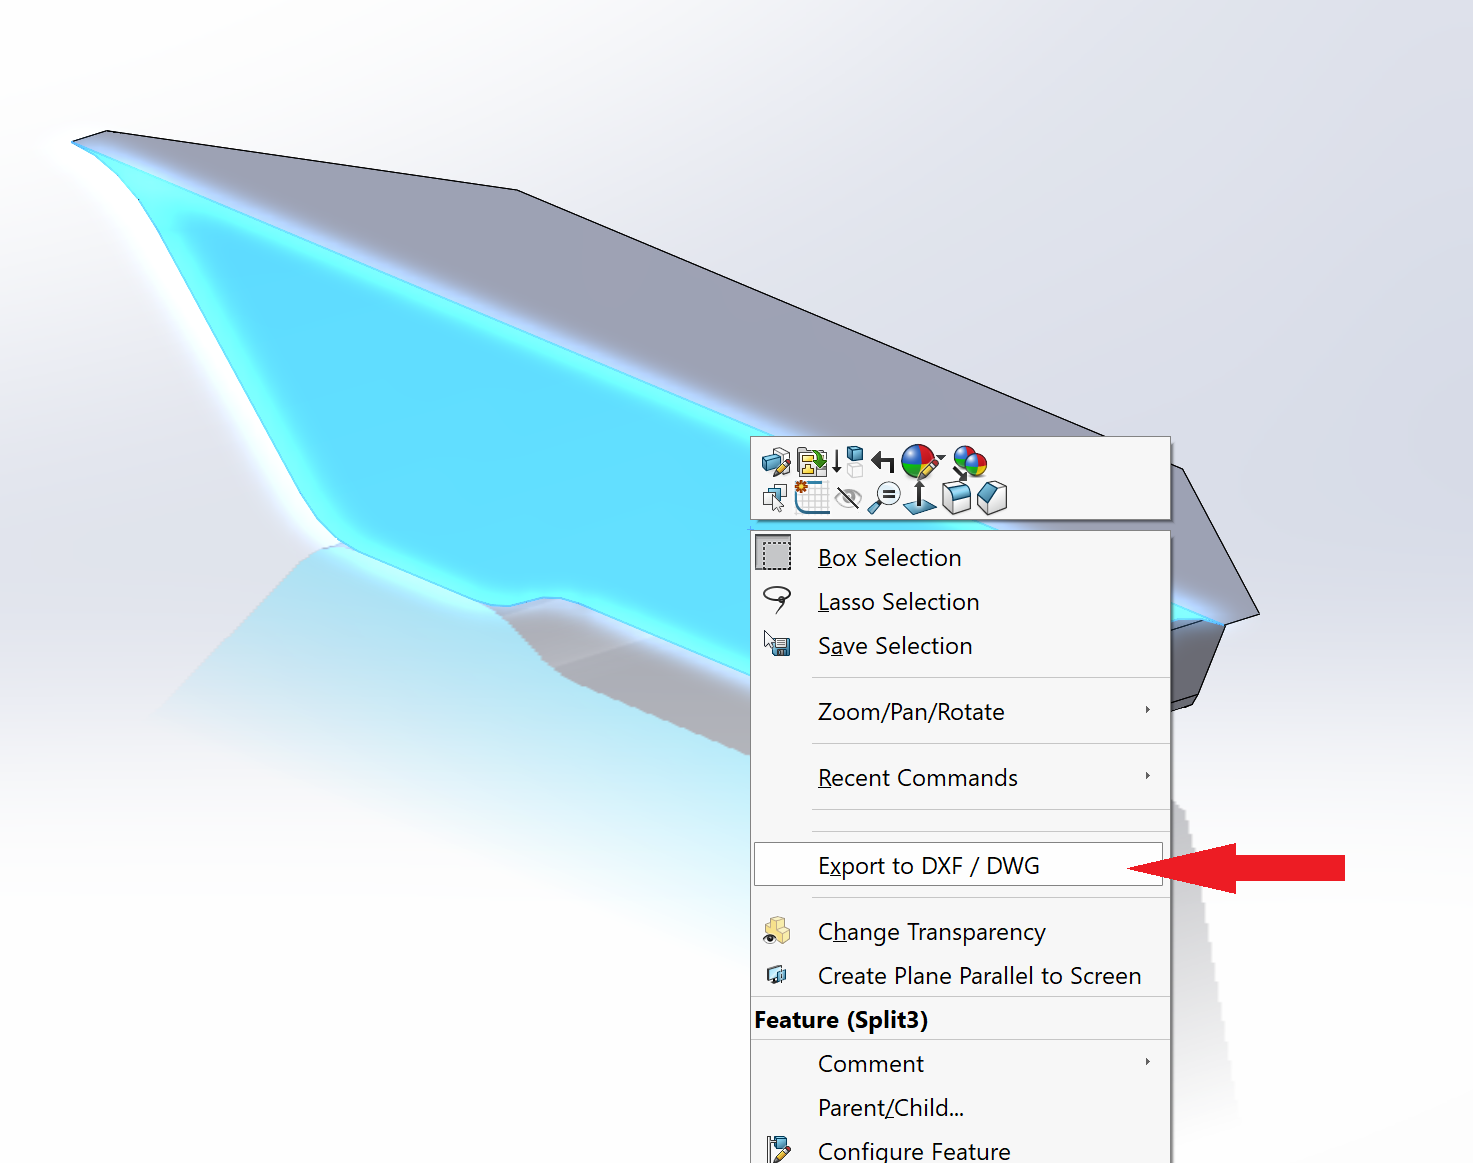
\includegraphics[width = 0.6\linewidth]{./Figures/general_shape/sw4.png}
			\caption{Export Side Profile}
			\label{fig:sw4}
		\end{figure}
		
		\item The top plane of the part is the projection from above, therefore, skip the split command and directly right click on the plane and export:
		\begin{figure} [H]
			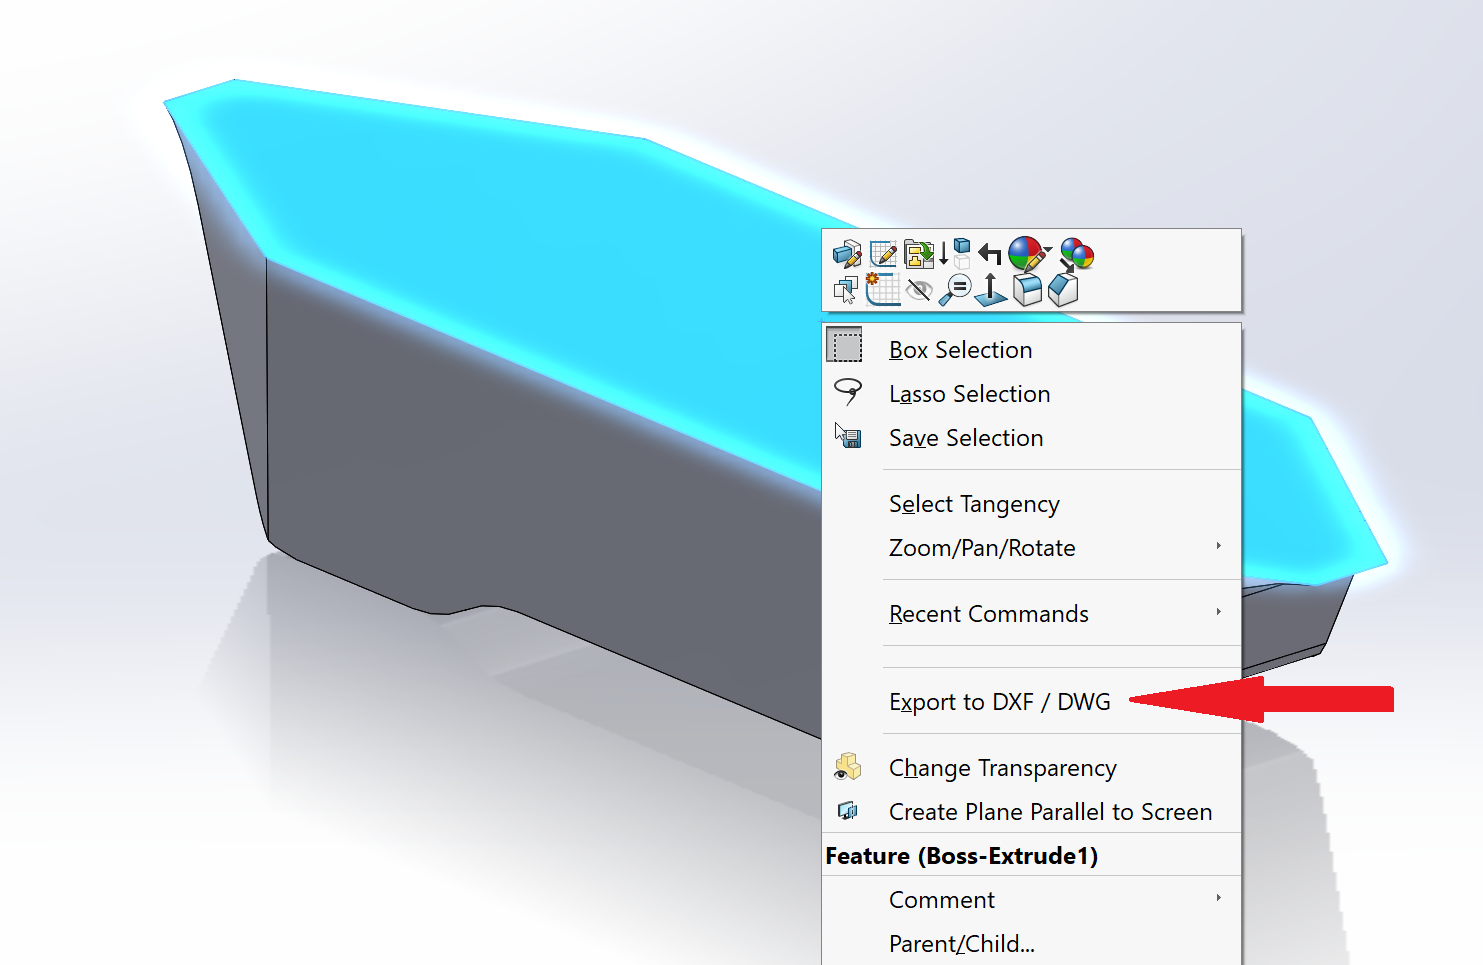
\includegraphics[width = 0.6\linewidth]{./Figures/general_shape/sw5.png}
			\caption{Export Top Profile}
			\label{fig:sw5}
		\end{figure}

	\end{itemize}
	
	\item Open AutoCAD, increase the precision by clicking the top left red AutoCAD sign, select ``Drawing Utilities $\rightarrow$ Units'' and increase the precision to 4 decimal points, as shown in fig~\ref{fig:cad1} below.
	\begin{figure}[H]
		\centering
		\begin{subfigure}[b]{.4\textwidth}
			\centering
			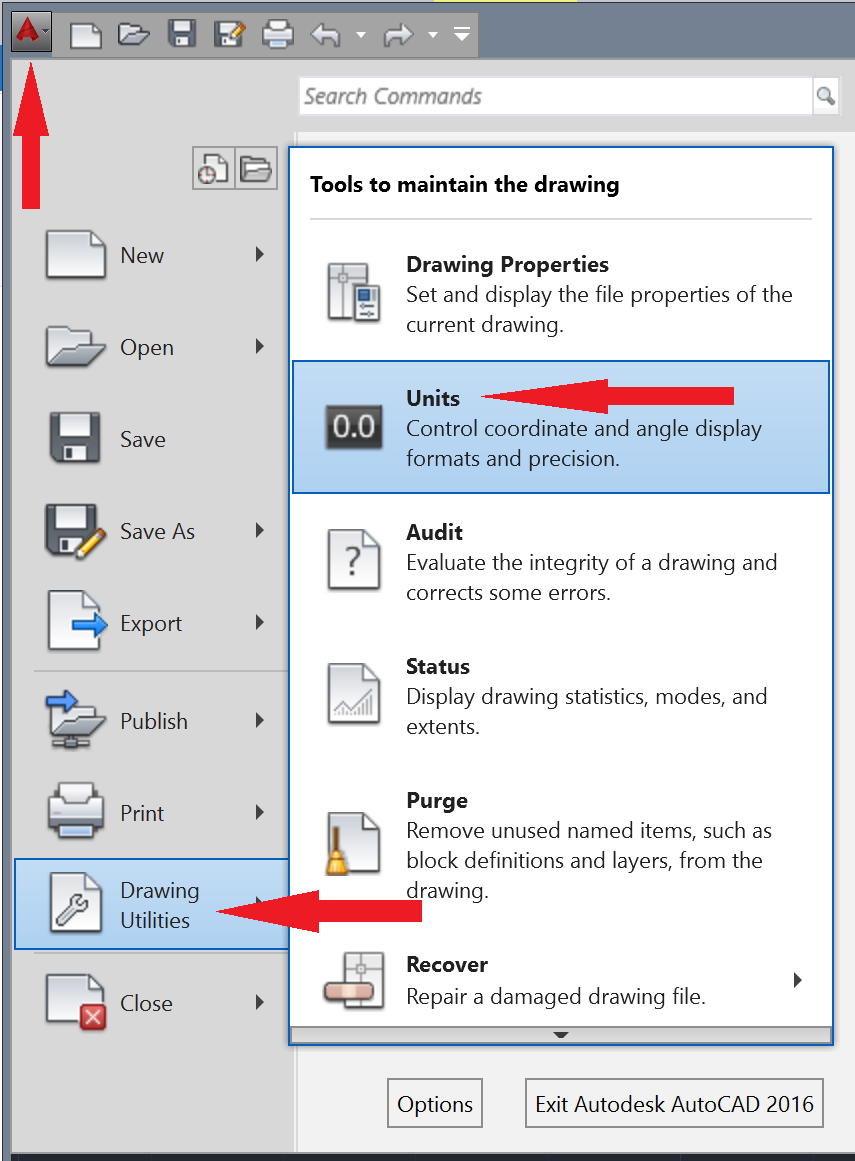
\includegraphics[width=\textwidth]{./Figures/general_shape/cad1.png}
		\end{subfigure}
		\begin{subfigure}[b]{.4\textwidth}
			\centering
			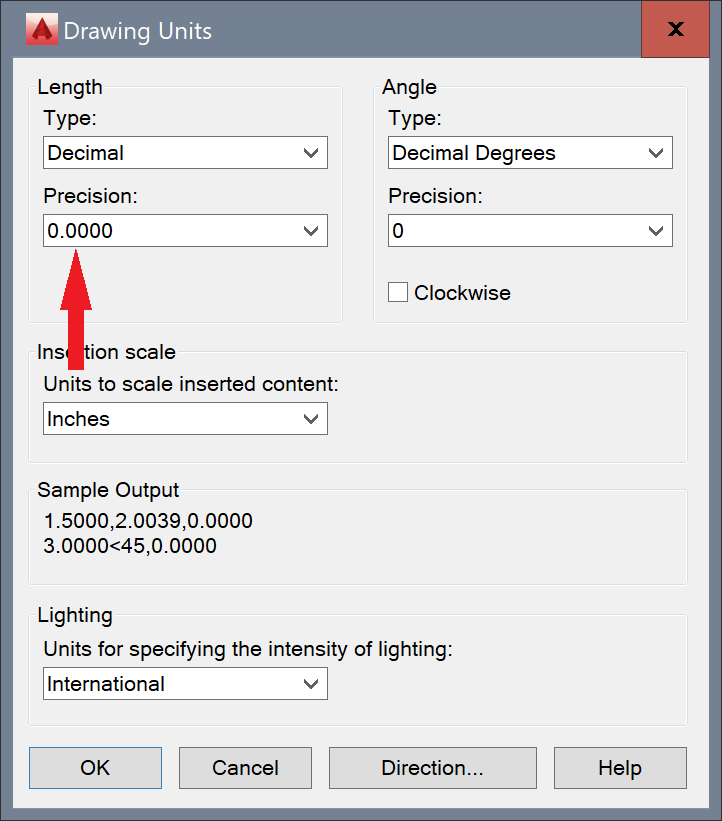
\includegraphics[width=\textwidth]{./Figures/general_shape/cad2.png}
		\end{subfigure}
		\caption{Increase AutoCAD Precision}
		\label{fig:cad1}
	\end{figure}
	
	\item Import the dxf files from SolidWorks.
	\item Scale the drawing by 25.4 if the SolidWorks file is in inches.
	\item Select all objects and run ``Explode'' command.
	\item Select all Spline (if any), right click and select ``Spline $\rightarrow$ Convert to Polyline'' as shown in fig~\ref{fig:cad3} below. When ask to enter accuracy, enter 1 and press enter.
	\begin{figure} [H]
		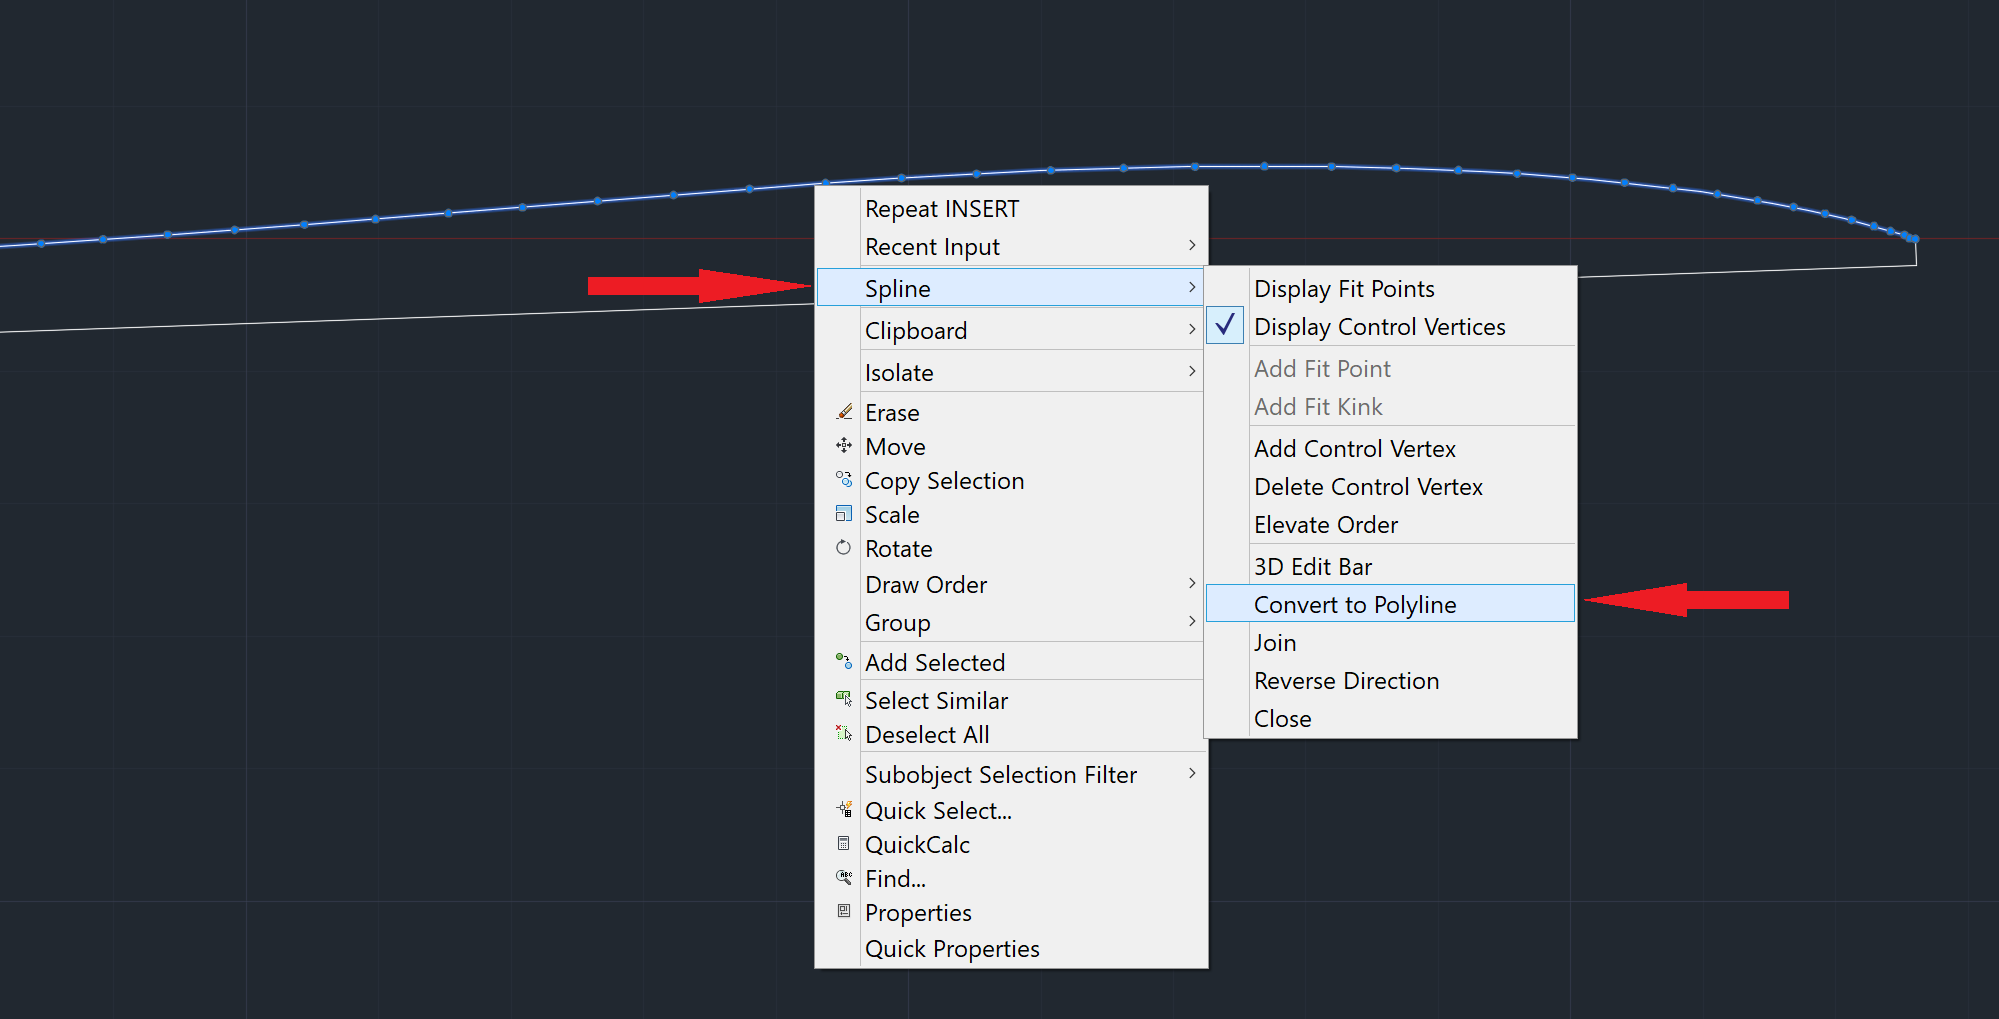
\includegraphics[width = 0.9\linewidth]{./Figures/general_shape/cad3.png}
		\caption{Convert Spline}
		\label{fig:cad3}
	\end{figure}
	\item Explode again (explode the polylines converted from spline).
	\item Rotate and delete overlapping lines if necessary.
	\item Select all lines and run ``eattext'' command, a window similar to fig~\ref{fig:cad4} should pop up, select ``Edit an existing data extraction'' then click the browse button.
	\begin{figure} [H]
		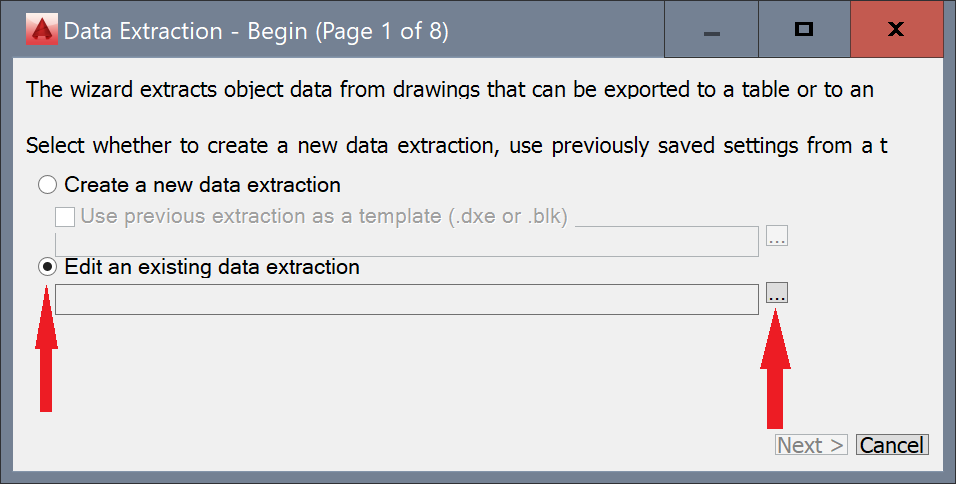
\includegraphics[width = 0.6\linewidth]{./Figures/general_shape/cad4.png}
		\caption{Eattext Page 1}
		\label{fig:cad4}
	\end{figure}
	\item Browse for the extraction templates, select the template with or without arc depending on the drawing. (The templates should be included with the manual package)
	\begin{figure} [H]
		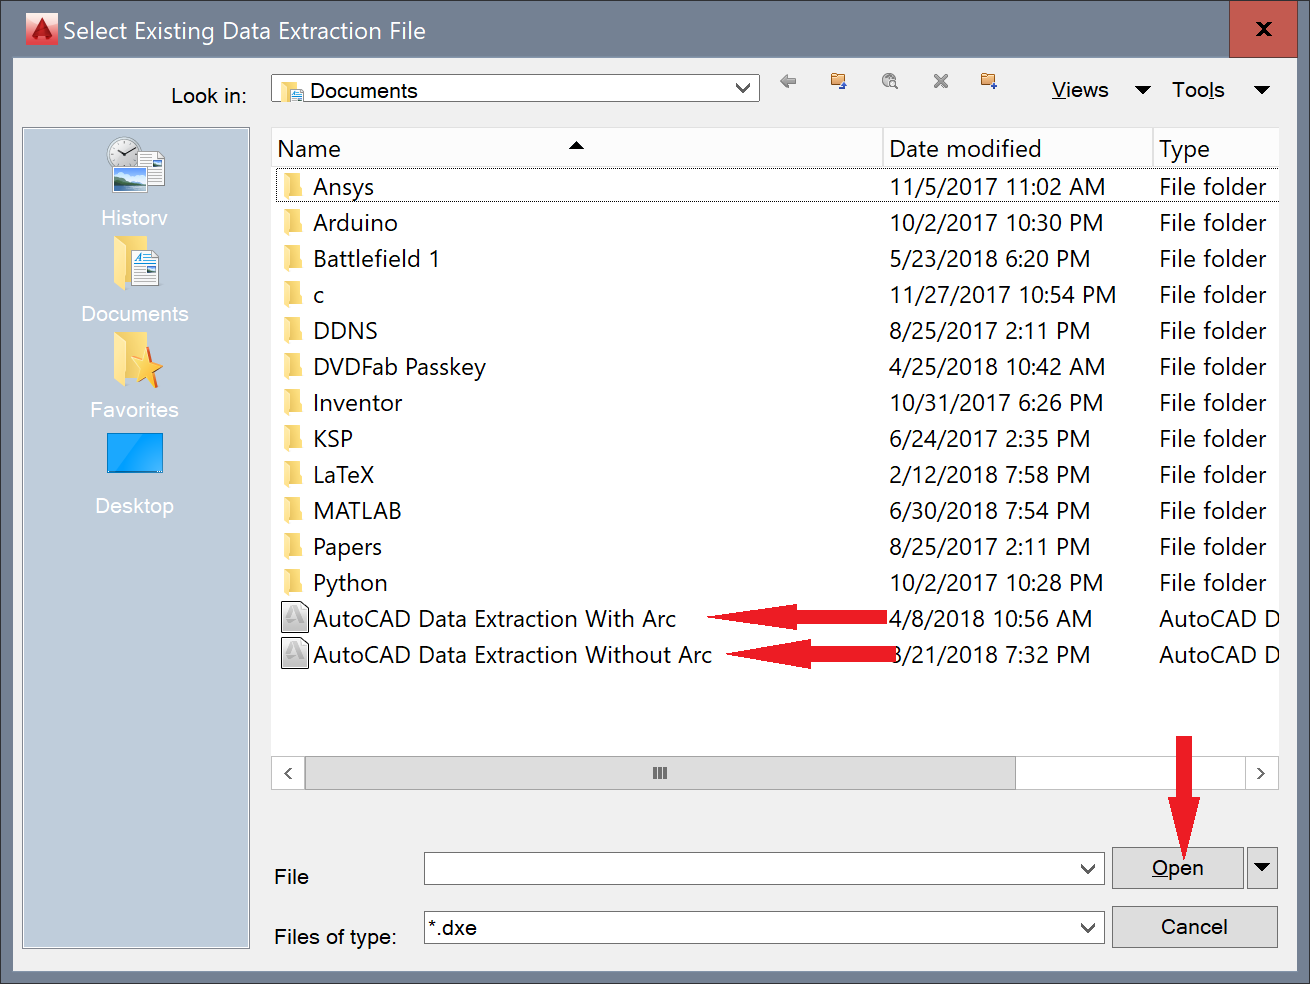
\includegraphics[width = 0.6\linewidth]{./Figures/general_shape/cad5.png}
		\caption{Browse for Data Extraction Templates}
		\label{fig:cad5}
	\end{figure}
	\item On page 2, check ``include current drawing'', select the one that is not the current drawing (if any) and click remove. 
	\begin{figure} [H]
		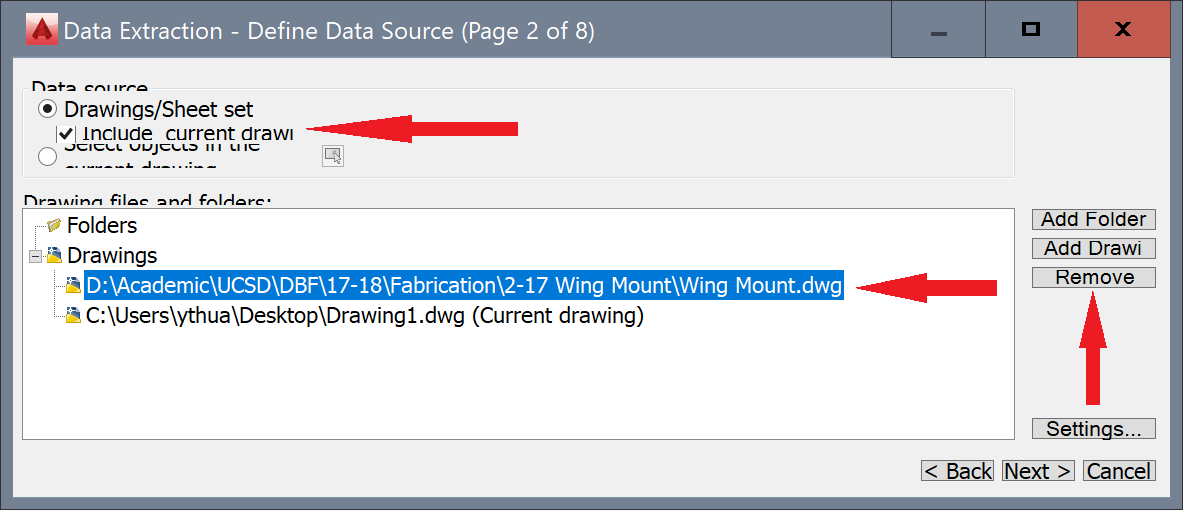
\includegraphics[width = 0.6\linewidth]{./Figures/general_shape/cad6.png}
		\caption{Eattext Page 2 Step 1}
	\end{figure}
	\item Then select the current drawing and click ``Next''.
	\begin{figure} [H]
		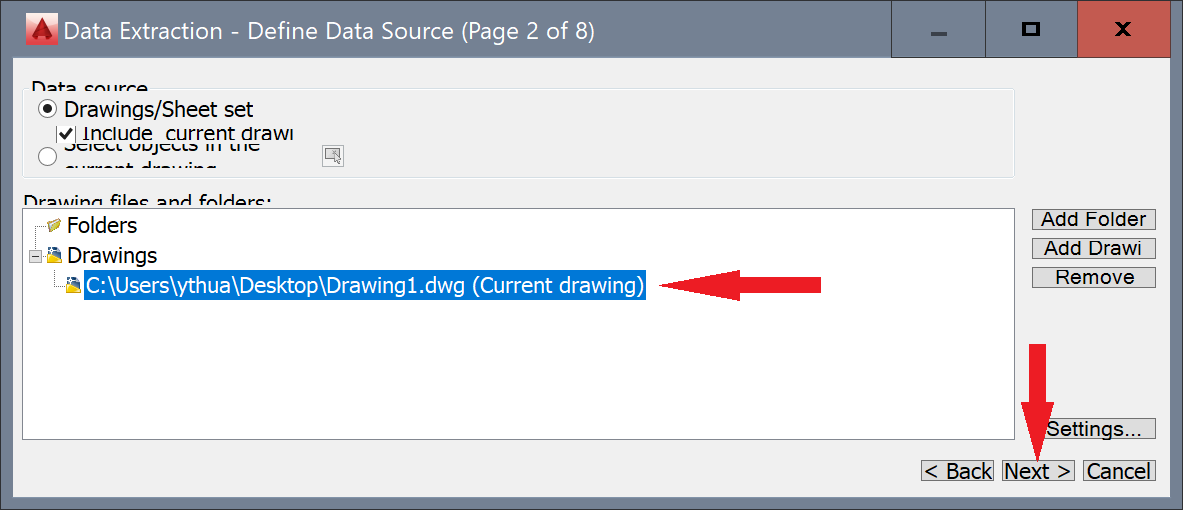
\includegraphics[width = 0.6\linewidth]{./Figures/general_shape/cad7.png}
		\caption{Eattext Page 2 Step 2}
	\end{figure}
	\item On page 3, make sure the drawing only has lines, or only has lines and arcs, depending on the template used. If not, cancel the process, fix the drawing, and redo the ``eattext'' command.
	\begin{figure} [H]
		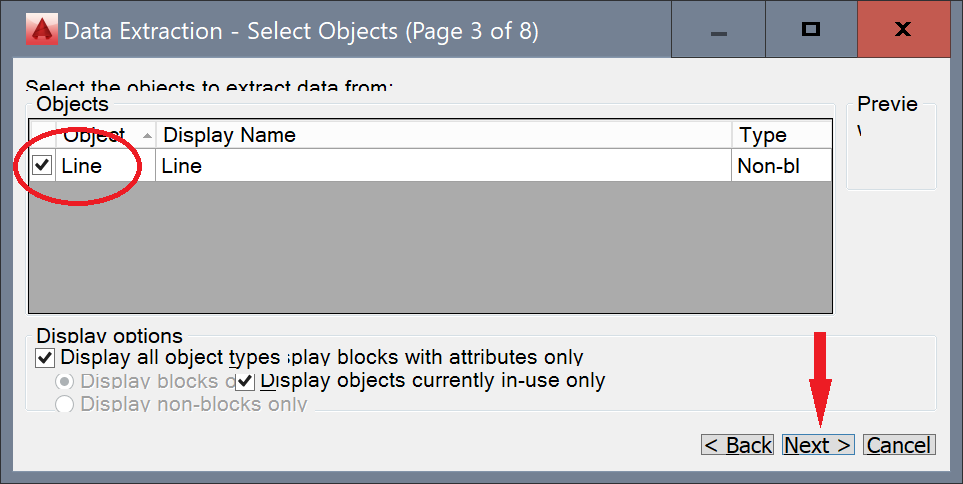
\includegraphics[width = 0.6\linewidth]{./Figures/general_shape/cad8.png}
		\caption{Eattext Page 3}
	\end{figure}
	
	\item Continue clicking ``Next'' until reaching page 6, name the data point file and save to the desired location. Click ``Next'' then ``Finish''.
	\begin{figure} [H]
		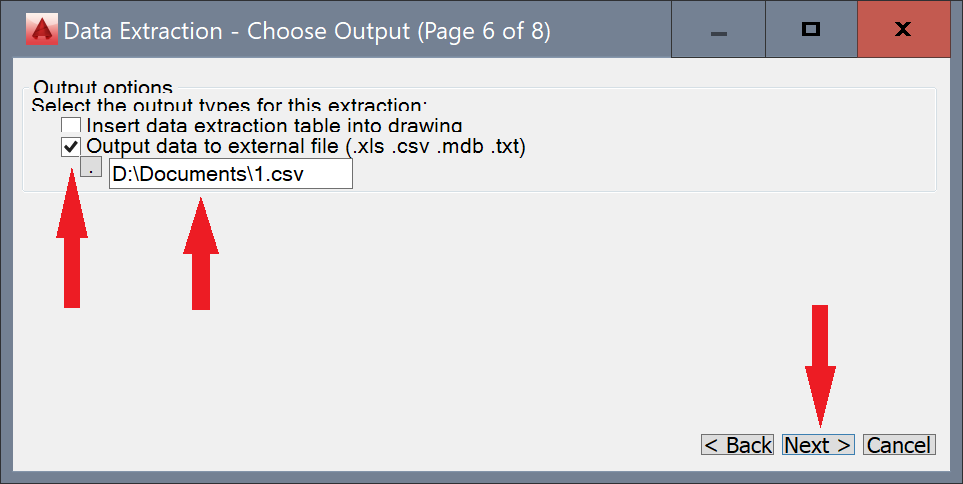
\includegraphics[width = 0.6\linewidth]{./Figures/general_shape/cad9.png}
		\caption{Eattext Page 6}
	\end{figure}

	\item Put the .csv file from AutoCAD into the same folder as the MatLAB scritpt ``DBF\_foamcutter\_general\_shape.m'' and run the MatLAB code. Follow the prompts, and the G-code should be ready.


\end{enumerate}


\section{FoamCutter Setup}

The entire foamcutter as shown in fig~\ref{fig:overview} below consists of two side frames each having two axis of motion, four 4-feet long connection rods, and a work panel for securing the foam. 

\begin{figure} [H]
	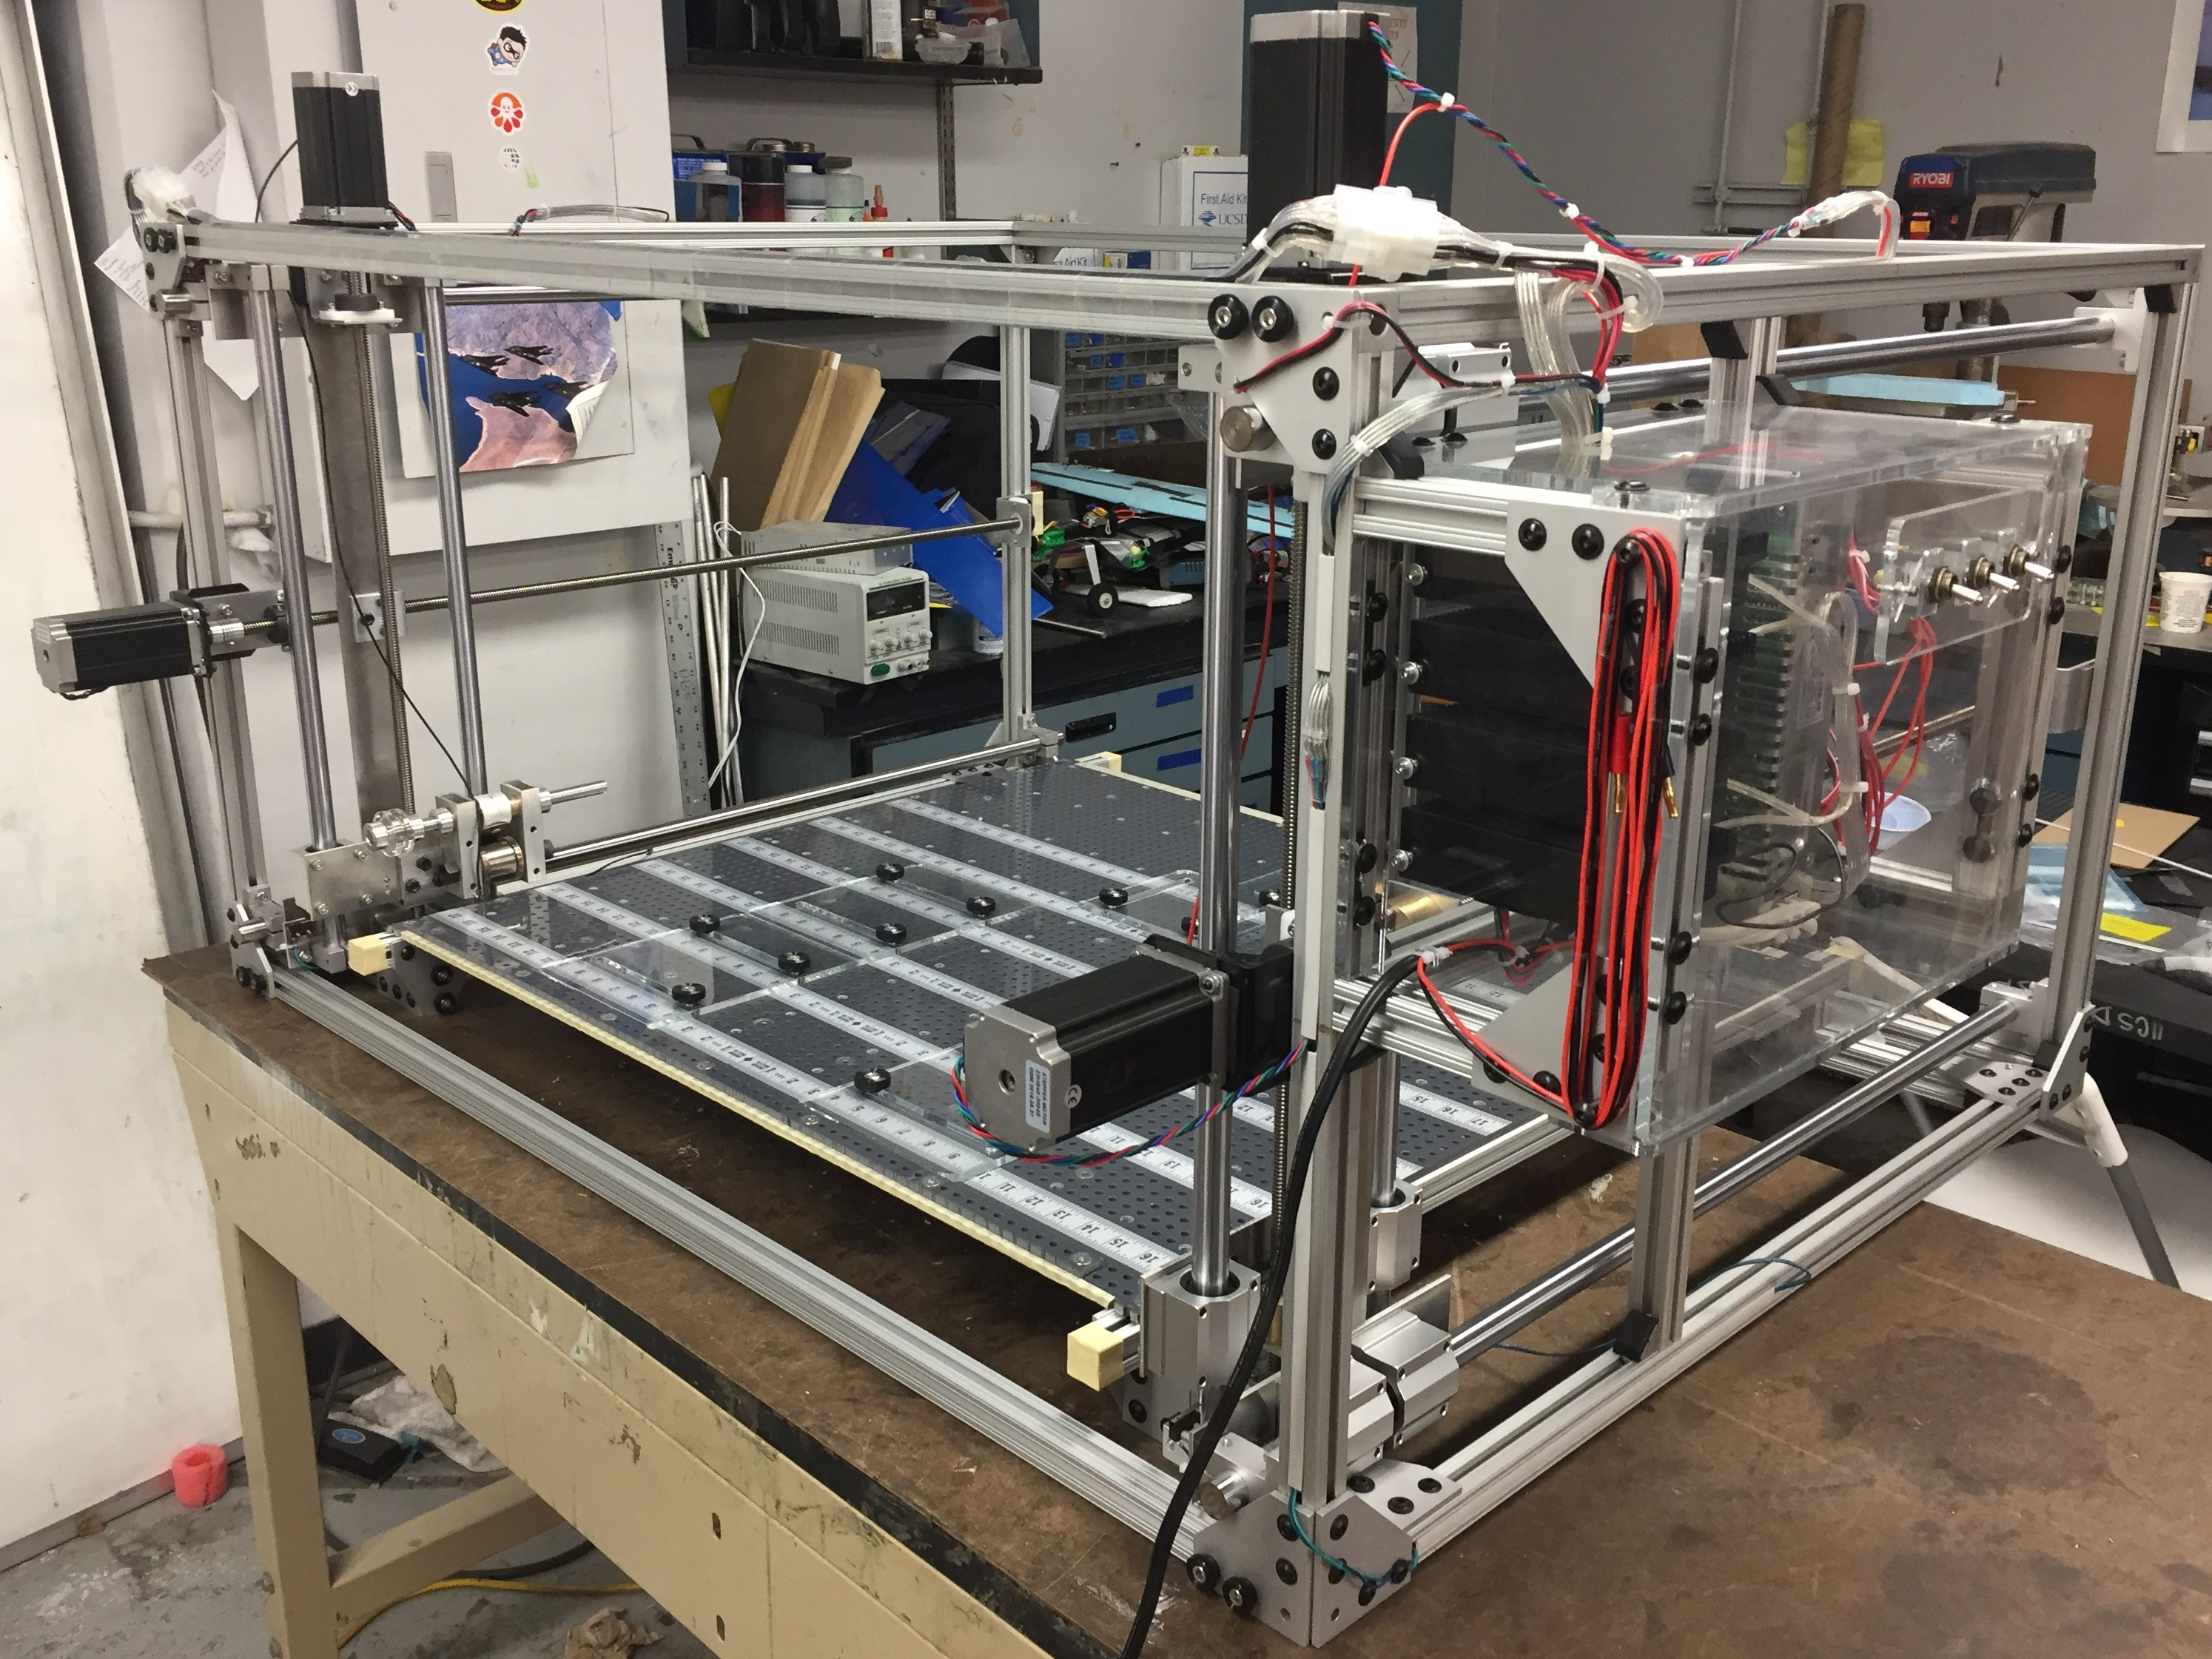
\includegraphics[width = 0.9\linewidth]{./Figures/overview.jpg}
	\caption{Foamcutter Overview}
	\label{fig:overview}
\end{figure}

\begin{tcolorbox}
	{\Large
\noindent Do:
\begin{itemize}[noitemsep,topsep=0pt]
	\item Always make sure the two side panels are connected with the connection rods;
	\item Always 
\end{itemize}

\noindent Don't:
\begin{itemize}[noitemsep,topsep=0pt]
	\item Never let the side panels stand on their own;
	\item Never over tighten the thumb screws on the work panel;
\end{itemize}
}
\end{tcolorbox}

\subsection{Connecting the two Side Panels}
The two side panels are connected with 4 connection rods, use the 4ft long connection rods for performing cutting and use the 2ft long connection rods (not purchased yet) for storage of the foamcutter. Each of the 4 connection rods are secured with two thumb screws at each end shown in fig~\ref{fig:thumb_screw}, loosen the thumb screws to remove the connection rod. 

\begin{figure} [H]
	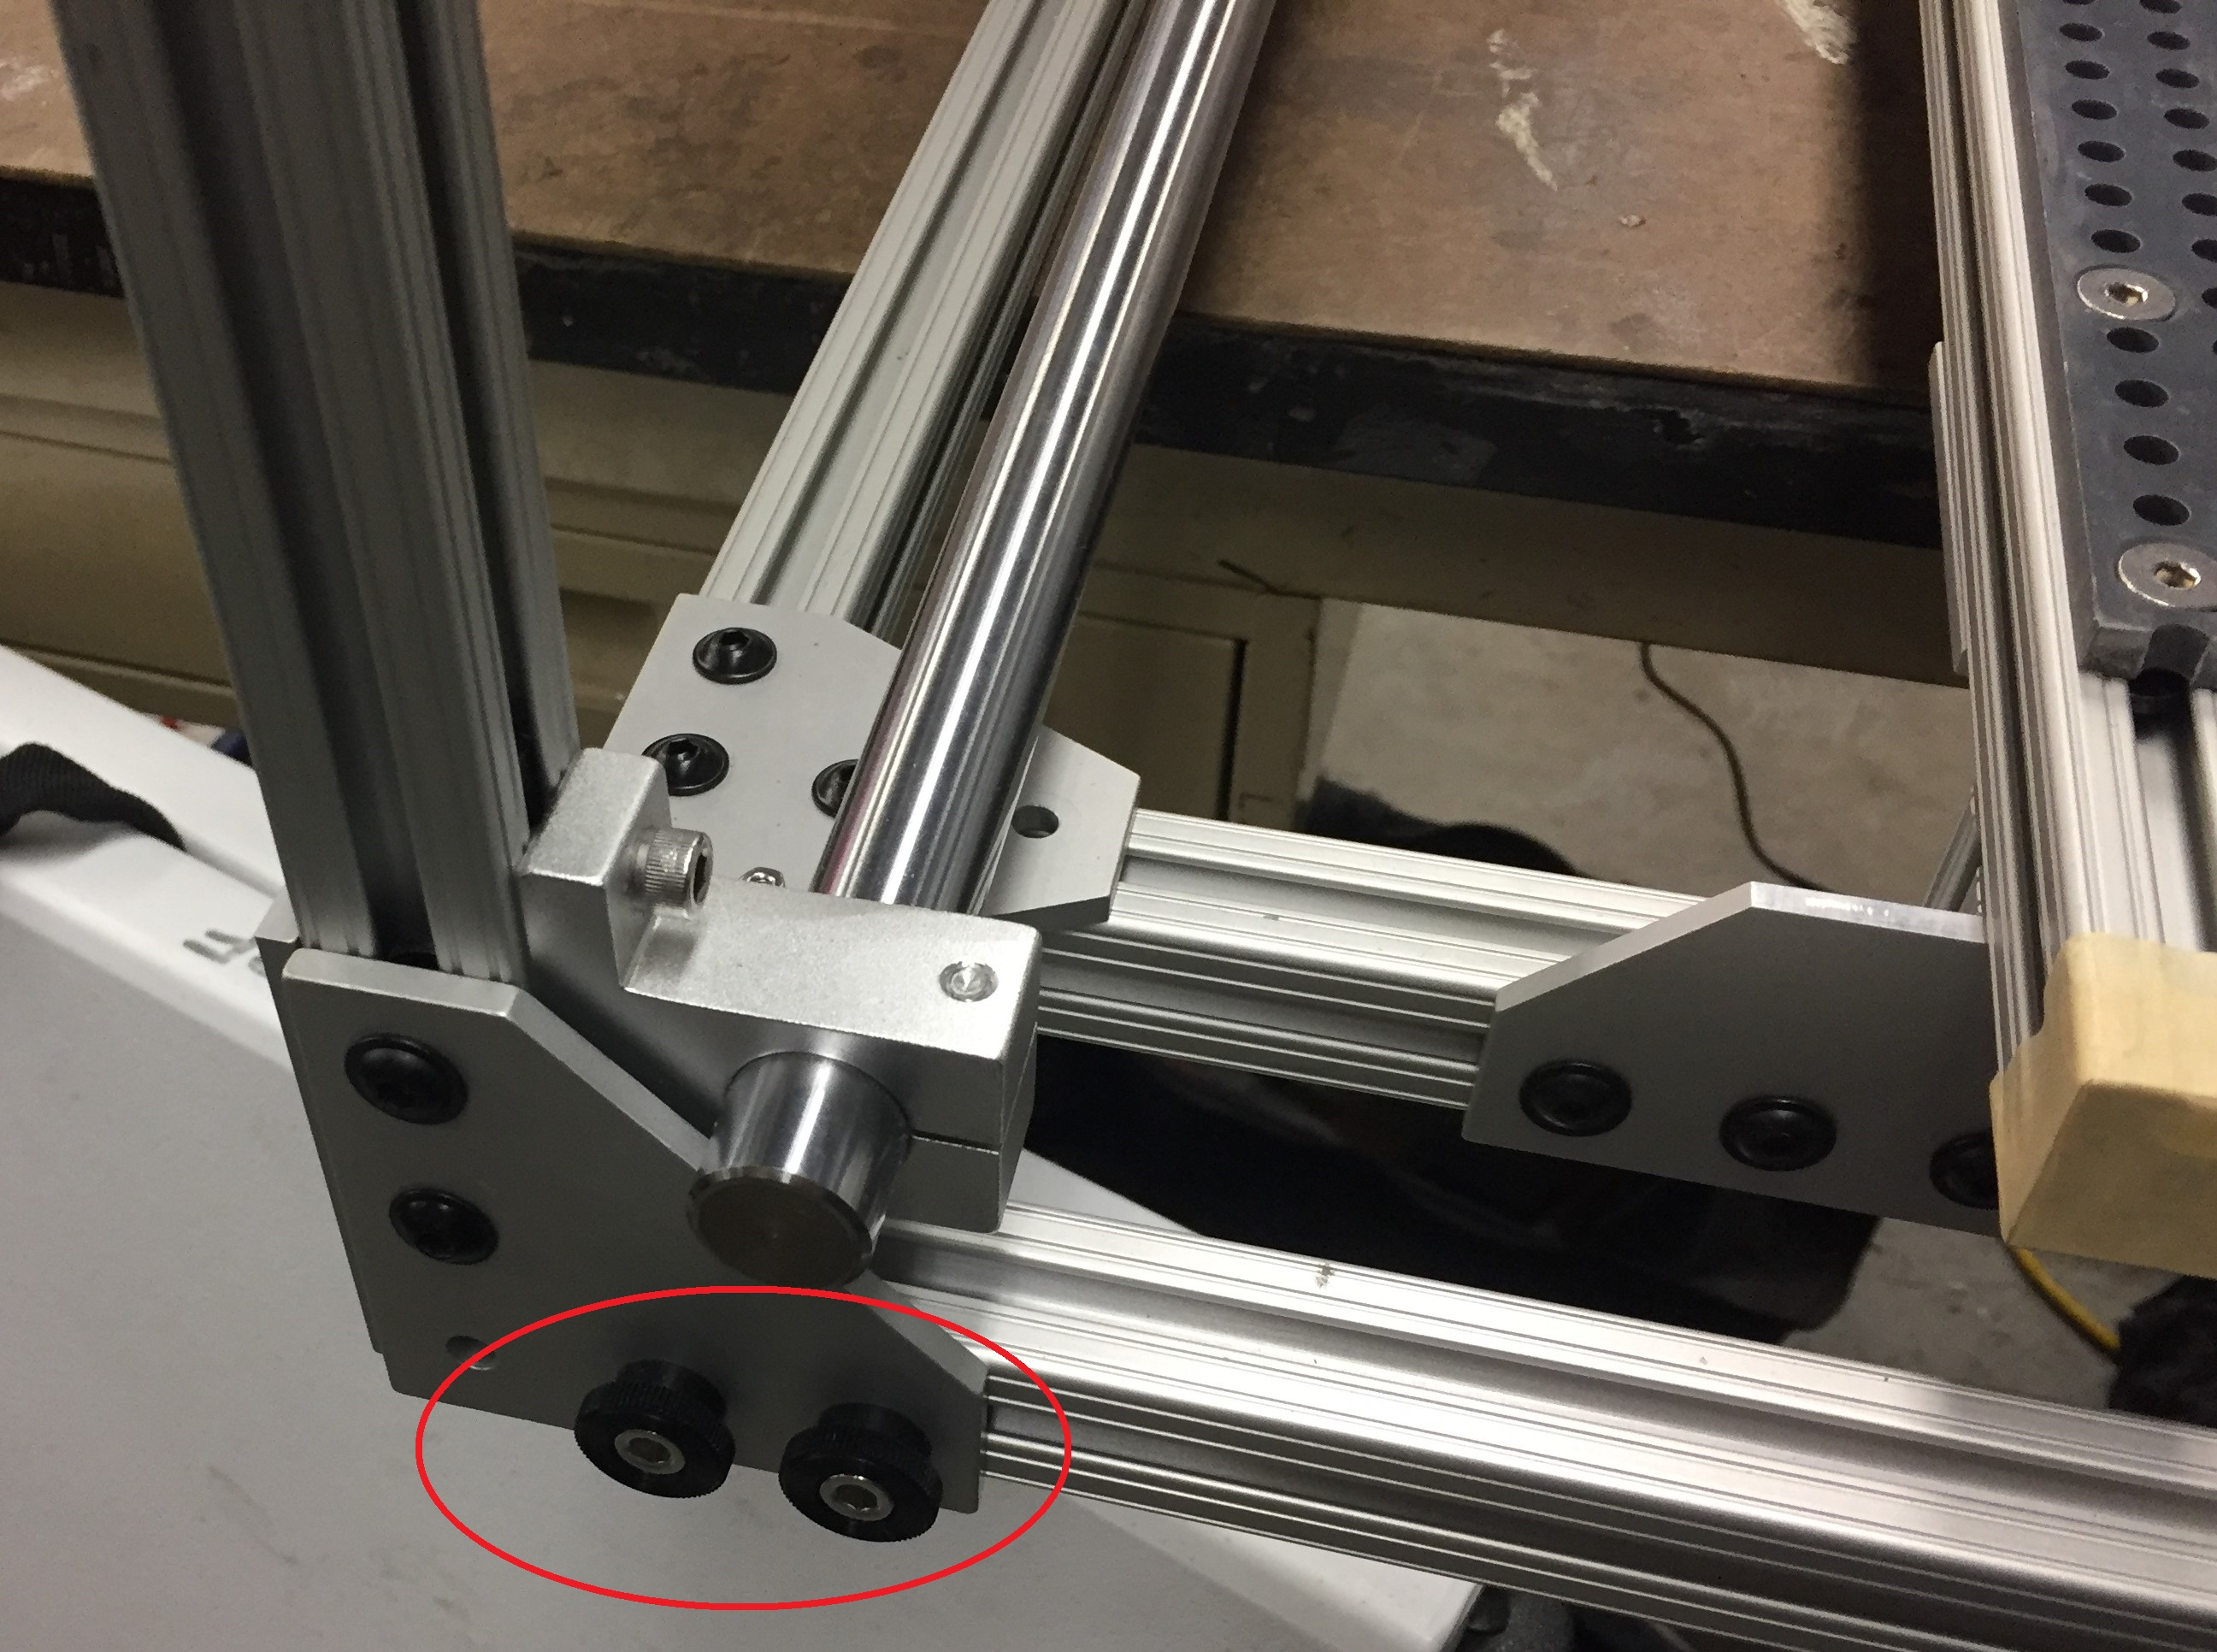
\includegraphics[width = 0.9\linewidth]{./Figures/thumb_screw.jpg}
	\caption{Thumb Screws for Connection Rods}
	\label{fig:thumb_screw}
\end{figure}

During the installation of the connection rods, do not let the side panels stand on their own. The side panels are capable of standing on their own, but are not designed to do so: deformation will occur and degrade the accuracy. When installing the connection rods, make sure there are no gaps between the frame and the connection rods then tighten the thumb screws. An Allen key is recommended to further tighten the thumb screws.

\subsection{Installing the Work Panel}



\newpage
\begin{appendices}
\chapter{Executive Summary}

\end{appendices}
\end{document}








%%%%%%%%%%%%%%%%%%%%%%%%%%%%%%%%%%%%%%%%%%%%%%%%%%
%%% Figures %%%%%%%%%%%%%%%%%%%%%%%%%%%%%%%%%%%%%%
%%%%%%%%%%%%%%%%%%%%%%%%%%%%%%%%%%%%%%%%%%%%%%%%%%
%\begin{figure} [H]
%	\includegraphics[width = \linewidth]{......}
%	\caption{......}
%\end{figure}
%%%%%%%%%%%%%%%%%%%%%%%%%%%%%%%%%%%%%%%%%%%%%%%%%%
%%% Subfigures %%%%%%%%%%%%%%%%%%%%%%%%%%%%%%%%%%%
%%%%%%%%%%%%%%%%%%%%%%%%%%%%%%%%%%%%%%%%%%%%%%%%%%
%\begin{figure}[H]
%	\centering
%	\begin{subfigure}[b]{.475\textwidth}
%		\centering
%		\includegraphics[width=\textwidth]{......}
%		\caption{......}
%	\end{subfigure}
%	\begin{subfigure}[b]{.475\textwidth}
%		\centering
%		\includegraphics[width=\textwidth]{......}
%		\caption{......}
%	\end{subfigure}
%	\centering
%	\begin{subfigure}[b]{.475\textwidth}
%		\centering
%		\includegraphics[width=\textwidth]{......}
%		\caption{......}
%	\end{subfigure}
%	\begin{subfigure}[b]{.475\textwidth}
%		\centering
%		\includegraphics[width=\textwidth]{......}
%		\caption{......}
%	\end{subfigure}
%	
%	\caption{......}
%\end{figure}
%%%%%%%%%%%%%%%%%%%%%%%%%%%%%%%%%%%%%%%%%%%%%%%%%%
%%% Tables %%%%%%%%%%%%%%%%%%%%%%%%%%%%%%%%%%%%%%%
%%%%%%%%%%%%%%%%%%%%%%%%%%%%%%%%%%%%%%%%%%%%%%%%%%
%\begin{table}[H]
%	\caption{......} 
%	\centering
%   \renewcommand{\arraystretch}{1.5}
%	\begin{tabular}{|c|m{20mm}|}  \hline
%		......& ...... \\ \hline
%		......&......  \\ \hline
%		......& ...... \\ \hline
%	\end{tabular} 
%\end{table}
%%%%%%%%%%%%%%%%%%%%%%%%%%%%%%%%%%%%%%%%%%%%%%%%%%
%%% Itemize %%%%%%%%%%%%%%%%%%%%%%%%%%%%%%%%%%%%%%
%%%%%%%%%%%%%%%%%%%%%%%%%%%%%%%%%%%%%%%%%%%%%%%%%%
%\begin{itemize}[noitemsep,topsep=0pt]
%	\item ......
%	\item ......
%\end{itemize}
%%%%%%%%%%%%%%%%%%%%%%%%%%%%%%%%%%%%%%%%%%%%%%%%%%
%%% Hyperlink %%%%%%%%%%%%%%%%%%%%%%%%%%%%%%%%%%%%
%%%%%%%%%%%%%%%%%%%%%%%%%%%%%%%%%%%%%%%%%%%%%%%%%%
%\href{url......}{displaytext......}
%%%%%%%%%%%%%%%%%%%%%%%%%%%%%%%%%%%%%%%%%%%%%%%%%%
%%% Code %%%%%%%%%%%%%%%%%%%%%%%%%%%%%%%%%%%%%%%%%
%%%%%%%%%%%%%%%%%%%%%%%%%%%%%%%%%%%%%%%%%%%%%%%%%%
%\newpage
%\appendix
%\section{MatLab code}
%\lstinputlisting{......}
%\section{C code}
%\includepdf[pages=-, pagecommand={}]{......}
%%%%%%%%%%%%%%%%%%%%%%%%%%%%%%%%%%%%%%%%%%%%%%%%%%
%%% Citation %%%%%%%%%%%%%%%%%%%%%%%%%%%%%%%%%%%%%
%%%%%%%%%%%%%%%%%%%%%%%%%%%%%%%%%%%%%%%%%%%%%%%%%%
%\bibliographystyle{plain}
%\bibliography{references}
%%%%%%%%%%%%%%%%%%%%%%%%%%%%%%%%%%%%%%%%%%%%%%%%%%
%%% Highlight %%%%%%%%%%%%%%%%%%%%%%%%%%%%%%%%%%%%
%%%%%%%%%%%%%%%%%%%%%%%%%%%%%%%%%%%%%%%%%%%%%%%%%%
%\hlcolor{yellow}{...}
